\documentclass[tikz,border=2pt]{standalone}
\usepackage{amsmath,amssymb}
\usepackage{pgfplots}
\pgfplotsset{compat=1.18}

\begin{document}
% Probability that at least two of n people share a birthday: it passes 50% already at
% n = 23 and is above 97% for n = 50.
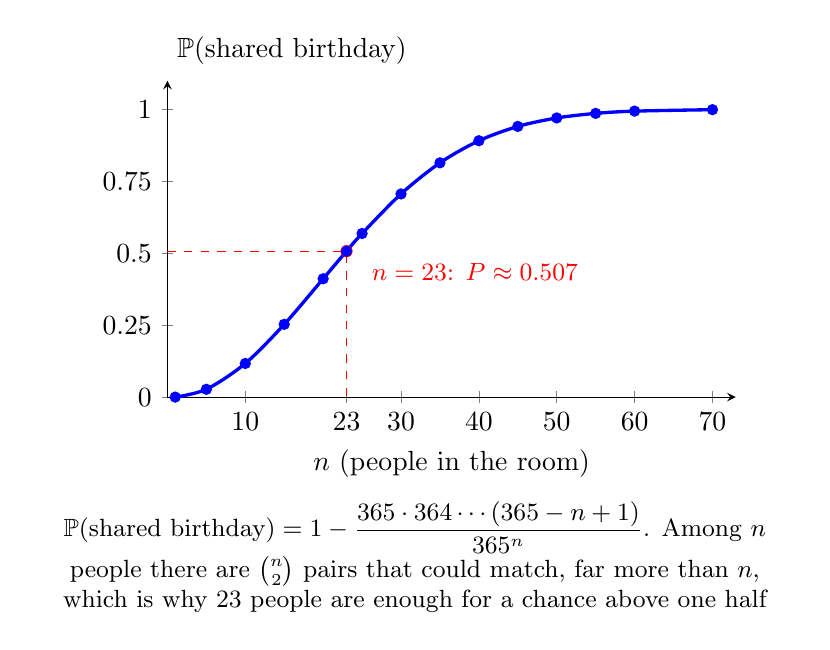
\begin{tikzpicture}
	\begin{axis}[
		axis lines=left, xmin=0, xmax=73, ymin=0, ymax=1.1,
		xtick={10,23,30,40,50,60,70}, ytick={0,0.25,0.5,0.75,1},
		xlabel={$n$ (people in the room)}, ylabel={$\mathbb{P}(\text{shared birthday})$}, ylabel style={rotate=-90, anchor=south west, at={(axis description cs:0,1.02)}},
		width=8.8cm, height=5.6cm, clip=false
		]
		\addplot[blue, very thick, smooth, mark=*, mark size=1.4pt] coordinates {(1,0) (5,0.0271) (10,0.1169) (15,0.2529) (20,0.4114) (23,0.5073) (25,0.5687) (30,0.7063) (35,0.8144) (40,0.8912) (45,0.9410) (50,0.9704) (55,0.9863) (60,0.9941) (70,0.9992)};
		\draw[red, dashed] (axis cs:0,0.5073) -- (axis cs:23,0.5073) -- (axis cs:23,0);
		\fill[red] (axis cs:23,0.5073) circle (2.2pt);
		\node[red, anchor=north west, font=\small] at (axis cs:25,0.5) {$n=23$: $P\approx0.507$};
	\end{axis}
	\node[anchor=north, font=\small, align=flush center, text width=9.6cm] at ([yshift=-2pt]current axis.outer south) {$\mathbb{P}(\text{shared birthday})=1-\dfrac{365\cdot364\cdots(365-n+1)}{365^n}$. Among $n$ people there are $\binom n2$ pairs that could match, far more than $n$, which is why $23$ people are enough for a chance above one half};
\end{tikzpicture}
\end{document}
